\documentclass[a4paper, 12pt]{article}
\usepackage[utf8]{inputenc}
\usepackage[russian,english]{babel}
\usepackage[T2A]{fontenc}
\usepackage[left=10mm, top=20mm, right=18mm, bottom=15mm, footskip=10mm]{geometry}
\usepackage{indentfirst}
\usepackage[yyyymmdd,hhmmss]{datetime}

\usepackage{titlesec}

\usepackage{graphicx}
\graphicspath{{images/}}
\DeclareGraphicsExtensions{.pdf,.png,.jpg}

\usepackage{wrapfig}
\usepackage{blindtext}
\usepackage{cmap}

\usepackage[x11names]{xcolor}

\usepackage{amsmath} %% math packages
\usepackage{amsfonts}
\usepackage{amsmath}
\usepackage{amssymb}
\usepackage{amsthm}
\usepackage{mathtools}

\usepackage{uniquecounter}
\usepackage{placeins}
\usepackage[italicdiff]{physics}
\usepackage{multirow}

\usepackage{hyperref} % links in document
\hypersetup{
    colorlinks=true,
    linkcolor=red,
    filecolor=magenta,      
    urlcolor=blue,
    pdftitle={Links},
    pdfpagemode=FullScreen,
}

\usepackage{import} %%inkspace images
\usepackage{xifthen}
\usepackage{pdfpages}
\usepackage{transparent}
\usepackage{caption}
\usepackage{fancyhdr}
\usepackage{type1cm}

\usepackage{caption}
\captionsetup[figure]{name=Рисунок}
\captionsetup[table]{name=Таблица}

\usepackage{fancyhdr}

\begin{document}

    %====================================================================================
\newcommand{\idLab}{0.0.0}
\newcommand{\authorLab}{Иванов И.И}
\newcommand{\authorGroup}{Б00-000}
\newcommand{\nameLab}{Смысл жизни}
\newcommand{\yearLab}{2000}
%====================================================================================
\definecolor{mycolor}{HTML}{671800}
\definecolor{default_color}{HTML}{FFFFFF}
\pagecolor{default_color}
%1)
%\pagestyle{fancy}
%\fancyhead{}
%\fancyfoot[C]{\color{default_color} \textit{\leftmark}}
%\renewcommand{\headrulewidth}{0pt}
%\fancypagestyle{plain}{
%  \renewcommand{\headrulewidth}{0pt}
%}
%2)
\pagecolor{white}
\pagestyle{fancy}
\fancyhf{}
\rhead{\textit{Отчет о выполненой лабораторной работе \idLab}}
\lhead{\textit{\authorLab}}
\rfoot{}

%\color{...} to make color text all
% Define custom colors
%\definecolor{cyanish}{RGB}{10,250,250}
%\definecolor{lightgreen}{HTML}{CCFF99}
%\definecolor{orangish}{wave}{620}
%\colorlet{ochre}{blue!30!yellow!70!}

\thispagestyle{empty}

\begin{center}
\large{«Московский физико-технический институт»} \\  
\vspace*{6cm}
{\bfseries
    {\Huge Отчёт о выполненной лабораторной работе \textnumero \idLab  \\ \nameLab}
}
\end{center}

\vspace*{1cm}
\begin{flushright}
    \large{
    \textbf{Выполнил:} \\ \textit{ \authorLab, \authorGroup} \\
    }
\end{flushright}

\vspace*{12cm}
\begin{center}
\yearLab
\end{center}

\newpage


    \section{Аннотация}

\underline{Цель работы}: 
\begin{enumerate}
    \item Изучение ВАХ тлеющего разряда.
    \item Изучение свойств плазмы методом зондовых характеристик.
\end{enumerate} \par
\underline{Оборудование}:
\par Стеклянная газоразрядная трубка, наполненная неоном; высоковольтный источник питания; источник питания постоянного тока; делитель напряжения; потенциометр; амперметры и вольтметры; переключатели.
\section{Теоретические сведения}
\par Плазма - ионизованный газ , дебаевский радиус которого $r_D$ существенно меньше характерного размера l объёма, занимаемого этим газом.
\par  Из-за теплового движения в плазме электроны могут смещаться относительно ионов и образовывать неоднородности. В этих неоднородностях возникает электрическое поле, которое стремится восстановить баланс, из-за чего происходят колебания с частотой 
\begin{equation}
 w_p = \sqrt{\frac{4\pi n_e e^2}{m_e}}
\end{equation}	
	За характерное время колебаний электроны за счет теплового движения смещаются на 
\begin{equation}
    r_D \sim \frac{v_e}{w_p} = \sqrt{\frac{kT_e}{4\pi n_e e^2}}
\end{equation}
	$r_D$ - дебаевский радиус, $k$ - константа Больцмана.\\
	Если поместить в плазму пробную (допустим, положительную) частицу, то электроны будут скапливаться около этой частицы, экранируя её поле. Потенциал точечного заряда будет иметь в плазме следующий вид:
	\[\varphi(r) = \frac{q}{r}e^{-\frac{r}{r_D}}\]
	где $r_D = \sqrt{\dfrac{kT_e}{4\pi n e^2}}$ -- \textit{радиус Дебая в случае равновесной плазмы}. Если температуры электронов и ионов сильно отличаются, то следует определять отдельно величину радиуса экранирования для электронов и для ионов. Итоговый радиус будет
	\[r_D = (r_{De}^{-2} + r_{Di}^{-2})^{-1/2}\]
	То есть если $T_i \ll T_e$, то $r_D \approx r_{Di}$ 
     Число заряженных частиц в сфере радиуса $r_D$:
     \begin{equation}
         N_D = \frac{4}{3}\pi n_i r^3_D
     \end{equation}


\subsection*{Одиночный зонд}
При внесении в плазму уединённого проводника -- \textit{зонда} -- с потенциалом, изначально равным потенциалу точки плазмы, в которую его помещают, на него поступают токи электроннов и ионов:
\begin{equation}
        I_{e0} = \dfrac{n \langle v_e \rangle}{4}eS,\\
\end{equation}
\begin{equation}
    I_{i0} = \dfrac{n \langle v_i \rangle}{4}eS,
\end{equation}
где $\langle v_e \rangle$ и $\langle v_i \rangle$ -- средние скорости электронов и ионов, $S$ -- площадь зонда, $n$ -- плотность электронов и ионов. Скорости электронов много больше скорости ионов, поэтому $I_{i0} \ll I_{e0}$. Зонд будет заряжаться до некоторого равновестного напряжения $-U_f$ -- \textit{плавающего потенциала}.\\
В равновесии ионный ток мало меняется, а электронный имеет вид
$$
I_e = I_0 \exp\left( -\dfrac{eU_f}{kT_e} \right).
$$
Будем подавать потенциал $U_\text{з}$ на зонд и снимать значение зондового тока $I_\text{з}$. Максимальное значение тока $I_{e\text{н}}$ -- электронный ток насыщения, а минимальное $I_{i\text{н}}$ -- ионный ток насыщения. Значение из эмпирической формулы Бомона:
\begin{equation}
    I_{i\text{н}} = 0.4 neS \sqrt{\dfrac{2kT_e}{m_i}}.
\end{equation}

Электронный ток насыщения можно определить по тепловому движению:
\[I_{e\text{н}} = \frac{n_eS}{4}\sqrt{\frac{8kT}{\pi m_e}}\]
\subsection*{Двойной зонд}
Двойной зонд -- система из двух одинаковых зондов, расположенных на небольшом расстоянии друг от друга, между которыми создаётся разность потенциалов, меньшая $U_f$. Рассчитаем ток между ними вблизи $I=0$. При небольших разностях потенциалов ионные токи на оба зонда близки к току насыщения и компенсируют друг друга, а значит величина результирующего тока полностью связана с разностью электронных токов. Пусть потенциалы на зондах
$$
U_1 = -U_f + \Delta U_1,
$$
$$
U_2 = -U_f + \Delta U_2.
$$
Между зондами $U = U_2 - U_1 = \Delta U_2 - \Delta U_1$.
Через первый электрод
\begin{equation}
    I_1 = I_{i\text{н}} + I_{e1} = I_{i\text{н}} - \dfrac{1}{4}neS\langle v_e\rangle \exp\left(-\dfrac{eU_f}{kT_e}\right)\exp\left(\dfrac{e\Delta U_1}{kT_e}\right)=I_{i\text{н}}\left(1 - \exp\left( \dfrac{e\Delta U_1}{kT_e} \right)\right).
\end{equation}
Аналогично через второй получим
\begin{equation}
    I_2 = I_{i\text{н}}\left(1 - \exp\left( \dfrac{e\Delta U_2}{kT_e} \right)\right)
\end{equation}

Из $(7)$ и $(8)$ с учётом последовательного соединение зондов ($I_1 = -I_2 = I)$:
$$
\Delta U_1= \dfrac{kT_e}{e}\text{ln}\left(1 - \dfrac{I}{I_{i\text{н}}}\right)
$$
$$
\Delta U_2= \dfrac{kT_e}{e}\text{ln}\left(1 + \dfrac{I}{I_{i\text{н}}}\right)
$$

Тогда итоговые формулы для разности потенциалов и тока

\begin{equation}
    U = \dfrac{kT_e}{e}\text{ln}\dfrac{1 - I/I_{i\text{н}}}{1 + I/I_{i\text{н}}}, \ \
    I = I_{i\text{н}} \text{th}\dfrac{eU}{2kT_e}.
\end{equation}
Из формулы можно найти формулу для $T_e$: для $U=0$ мы найдём $I_{i\text{н}}$, продифференцируем в точке $U=0$ и с учётом $\text{th}~\alpha \approx \alpha$ при малых $\alpha$ и $A\rightarrow 0$ получим:
\begin{equation}
    kT_e = \dfrac{1}{2}\dfrac{eI_{i\text{н}}}{\dfrac{dI}{dU}|_{U=0}}.
\end{equation}

\section*{Описание установки}
\begin{center}
    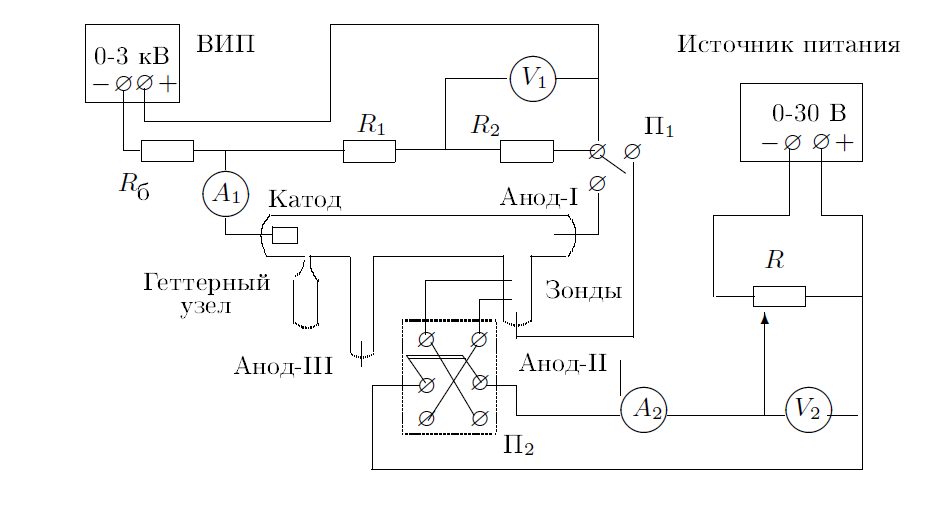
\includegraphics[scale=0.4]{setup.png}
\end{center}
\par Стеклянная газоразрядная трубка имеет холодный (ненакаливаемый) полый катод, три анода и \textit{геттерный} узел -- стеклянный баллон, на внутреннюю повехность которого напылена газопоглощающая плёнка (\textit{геттер}). Трубка наполнена изотопом неона $^{22}$Ne при давлении 2 мм рт. ст. Катод и один из анодом (I и II) с помощью переключателя $\Pi_1$ подключается через балластный резистор $R_\text{б}$ ($\approx 450$ кОм) к регулируемому ВИП с выкодным напряжением до 5 кВ.\\
При подключении к ВИП анода-I между ним и катодом возникает газовый разряд. Ток разряда измеряется миллиамперметром $A_1$, а падение напряжения на разрядной трубке -- цифровым вольтметром $V_1$, подключённым к трубке черезе высокоомный (25 МОм) делитель напряжения с коэффициентом $(R_1+R_2)/R_2 = 10$. \\
При подключении к ВИП анода-II разряд возникает в пространстве между катодом и анодом-II, где находятся двойной зонд, используемый для диагностики плазмы положительного столба. Зонды изготовлены из молибденовой проволоки диаметром $d = 0.2$ мм и имеют длину $l = 5.2$ мм. Они подключены к источнику питания GPS через потенциометр $R$. Переключатель $\Pi_2$ позволяет изменять полярность напряжения на зондах. Величина напряжения на зондах изменяеься с помощью дискретного переключателя <<$V$>> выходного напряжения источника питания и потенциометра $R$, а измеряется цифровым вольтметром $V_2$. Для измерения зондового тока используется мультиметр $A_2$.

\newpage
\section{Результаты эксперимента}
\begin{enumerate}
    \item  Определим напряжение зажигания:
    \begin{table}[!ht]
    \centering
    \begin{tabular}{|c|c|c|c|c|c|}
    \hline
    Vзаж, В & 93 & 103 & 95 & 105 & 110 \\ \hline
    \end{tabular}
    \caption{Напряжение зажигания}
    \end{table}
    $V_{заж} =$ 101 $\pm$ 6 В
    \item ВАХ разряда: в режиме переключателя $\text{П}_1$ снимем вольт-амперную характеристику разряда $I_p(U_p)$:
\begin{table}[!ht]
\centering
\begin{tabular}{|c|c|c|c|c|c|c|c|c|c|}
\cline{1-9}
$V_1 \text{В}$  & $I_1 \text{мА}$ &$ I_1 \text{мА}$ & $V_1 \text{В}$ &  & $I_1 \text{мА}$ &$ V_1 \text{В}$ & $I_1 \text{мА}$ & $V_1 \text{В}    $           \\ \cline{1-9}
25,50  & 2,10    & 3,02    & 22,20  &  & 3,92    & 16,70  & 2,91    & 22,60                \\ \cline{1-9}
25,10  & 2,22    & 3,09    & 21,80  &  & 3,84    & 17,20  & 2,80    & 22,90                \\ \cline{1-9}
24,90  & 2,26    & 3,16    & 21,50  &  & 3,80    & 17,40  & 2,69    & 23,40                \\ \cline{1-9}
24,70  & 2,35    & 3,23    & 21,10  &  & 3,73    & 17,90  & 2,61    & 23,60                \\ \cline{1-9}
24,50  & 2,39    & 3,32    & 20,60  &  & 3,66    & 18,40  & 2,56    & 23,80                \\ \cline{1-9}
24,40  & 2,44    & 3,41    & 20,00  &  & 3,60    & 18,80  & 2,52    & 23,90                \\ \cline{1-9}
24,20  & 2,47    & 3,53    & 19,30  &  & 3,54    & 19,20  & 2,48    & 24,10                \\ \cline{1-9}
24,00  & 2,52    & 3,60    & 18,80  &  & 3,46    & 19,80  & 2,41    & 24,30                \\ \cline{1-9}
23,70  & 2,62    & 3,65    & 18,50  &  & 3,35    & 20,40  & 2,32    & 24,60                \\ \cline{1-9}
23,60  & 2,66    & 3,72    & 18,10  &  & 3,28    & 20,80  & 2,23    & 24,70                \\ \cline{1-9}
23,50  & 2,70    & 3,82    & 17,40  &  & 3,20    & 21,20  &         &                      \\ \cline{1-9}
23,00  & 2,86    & 3,85    & 17,20  &  & 3,11    & 21,70  &         & \multicolumn{1}{l|}{} \\ \cline{1-9}
22,50  & 2,94    & 3,92    & 16,70  &  & 3,00    & 22,20  &         & \multicolumn{1}{l|}{} \\ \cline{1-9}
\end{tabular}
\caption{ВАХ при нарастании и убывании тока}
\end{table}

\begin{figure}[h!]
    \centering
    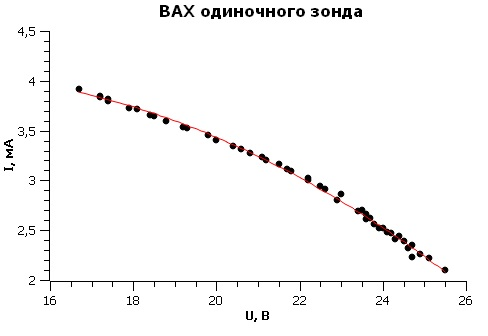
\includegraphics[scale=1.4]{ВАХ_1.jpg}
    \caption{ВАХ одиночного зонда}
    \label{fig:ref_to_this_foto}
\end{figure}

По этому графику определим максимальное дифференциальное сопротивление разряда:
$R_{\text{диф}} = \frac{dU}{dI} = -10.5 \pm 0.7 \text{кОм}$. Такое поведение ВАХ  соответствует участку поднормальному тлеющему заряду теоретической зависимости.

    \item Двойной зонд: измерим ВАХ двойного зонда $I_3(U_3)$ при $I_p$ = 4,04 мА, 2,99 мА и 2,31 мА.
    Далее при расчётах $I_1$ = 4.04 мА, $I_2$ = 2.99 мА, $I_3$ = 2.31 мА, $n_e = n_i = n$.


\begin{table}[h!]
\centering
\begin{tabular}{|c|c|c|c|c|c|}
\hline
$U_1$, В   & $I_1$, мкрА & $U_2$, В  & $I_2$, мкрА & $U_3$, В  & $I_3$, мкрА \\ \hline
25,00   & 41,90    & 24,87  & 29,5     & 24,87  & 23,26    \\ \hline
22,70   & 40,40    & 22,033 & 28,85    & 22,06  & 22,7     \\ \hline
21,90   & 40,00    & 19,01  & 28,15    & 18,93  & 22,03    \\ \hline
19,00   & 39,10    & 15,96  & 27,4     & 16,02  & 21,3     \\ \hline
16,03   & 38,17    & 13,01  & 26,48    & 12,98  & 20,44    \\ \hline
13,05   & 36,96    & 10,01  & 24,95    & 9,96   & 19,03    \\ \hline
9,97    & 34,76    & 7,94   & 22,92    & 8,02   & 17,46    \\ \hline
8,03    & 32,12    & 6,06   & 19,9     & 6,01   & 14,96    \\ \hline
6,01    & 27,57    & 4,04   & 15,03    & 4,04   & 11,3     \\ \hline
3,99    & 20,82    & 1,99   & 8,46     & 2,06   & 6,5      \\ \hline
2,02    & 12,24    & 0,01   & 1,27     & 0,01   & 0,8      \\ \hline
0,70    & 4,01     & -2,02  & -6,74    & -2,01  & -5,13    \\ \hline
-2,041  & -9,56    & -4,02  & -11,91   & -4,05  & -9,17    \\ \hline
-4,007  & -16,6    & -5,99  & -15,33   & -5,98  & -11,76   \\ \hline
-6,07   & -21,6    & -8,07  & -17,44   & -8,04  & -13,44   \\ \hline
-8,08   & -24,4    & -10,09 & -18,58   & -10,03 & -14,4    \\ \hline
-10,043 & -25,9    & -13,11 & -19,5    & -12,98 & -15,25   \\ \hline
-12,99  & -27,2    & -15,99 & -20,01   & -16,06 & -15,85   \\ \hline
-14,98  & -27,78   & -18,87 & -20,56   & -18,97 & -16,33   \\ \hline
-18,056 & -28,56   & -22,03 & -21,24   & -21,99 & -16,8    \\ \hline
-21,079 & -29,25   & -24,87 & -21,75   & -24,87 & -17,5    \\ \hline
\end{tabular}
\caption{ВАХ двойного зонда при $I_p$  = 4.04; 2,99; 2,31 мА}
\end{table}
\newpage
\subsection{Построим общий график}:
\begin{figure}[h!]
    \centering
    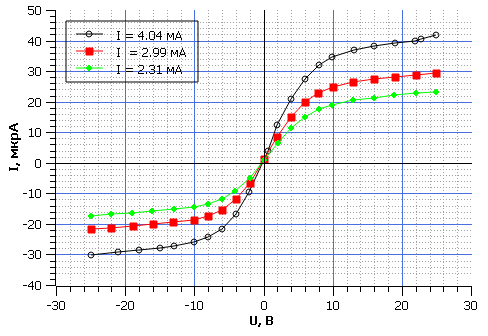
\includegraphics[scale=1.2]{ВАХ_2.png}
    \caption{ВАХ двойного зонда}
    \label{fig:ref_to_this_foto}
\end{figure}

\subsection{И отдельно найдём токи насыщения и температуры электронов в плазме}
\begin{figure}[h!]
    \centering
    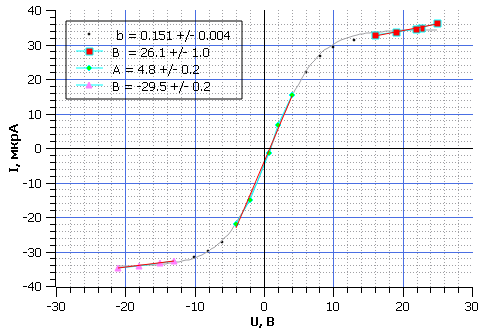
\includegraphics[scale=1.2]{ВАХ_404.png}
    \caption{ВАХ при $I_p$ = 4.04 мА}
    \label{fig:ref_to_this_foto}
\end{figure}

\par $1) \frac{dI}{dU} = (4.3 \pm 0.2) \cdot 10^6 \text{ См (Сименс)}$;
    $I_{\text{нас}} = (8.3 \pm 0.2) \cdot 10^4 \text{ СГСэ}$. \newline
Их температуры соответственно: $(6.6 \pm 0.3) \cdot 10^4 K \approx (5.7 \pm 3) \text{ эВ}$.
Согласно формуле (2) $n_i = $

\begin{figure}[h!]
    \centering
    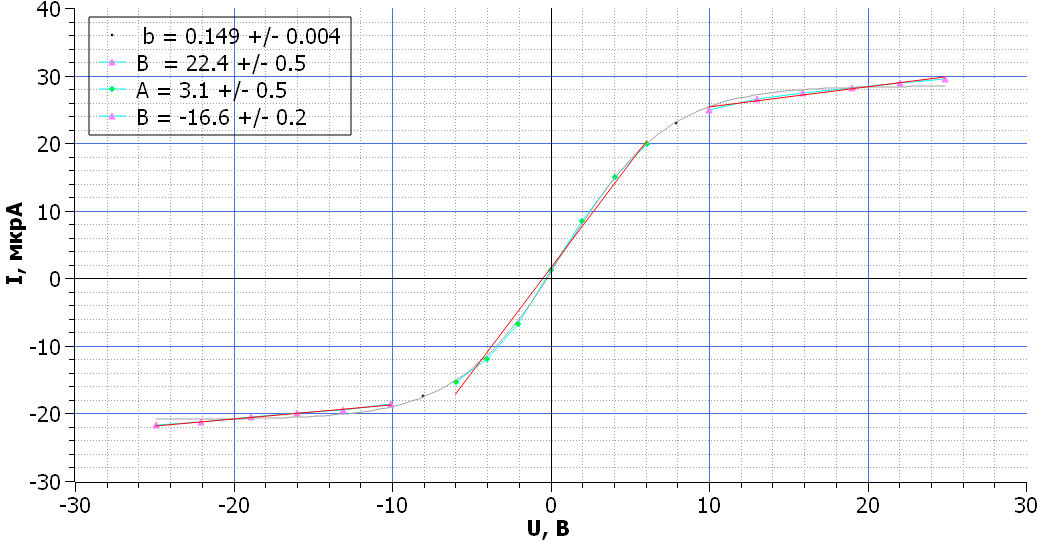
\includegraphics[scale=0.7]{ВАХ_299.png}
    \caption{ВАХ при $I_p$ = 2.99 мА}
    \label{fig:ref_to_this_foto}
\end{figure}

\par $2) \frac{dI}{dU} = (2.8 \pm 0.5) \cdot 10^6 \text{ См (Сименс)}$;
    $I_{\text{нас}} = (5.9 \pm 0.1) \cdot 10^4 \text{ СГСэ}$. \newline
Их температуры соответственно: $(3.7 \pm 0.7) \cdot 10^4 K \approx (3.2 \pm 0,6) \text{ эВ}$
\newline
\begin{figure}[h!]
    \centering
    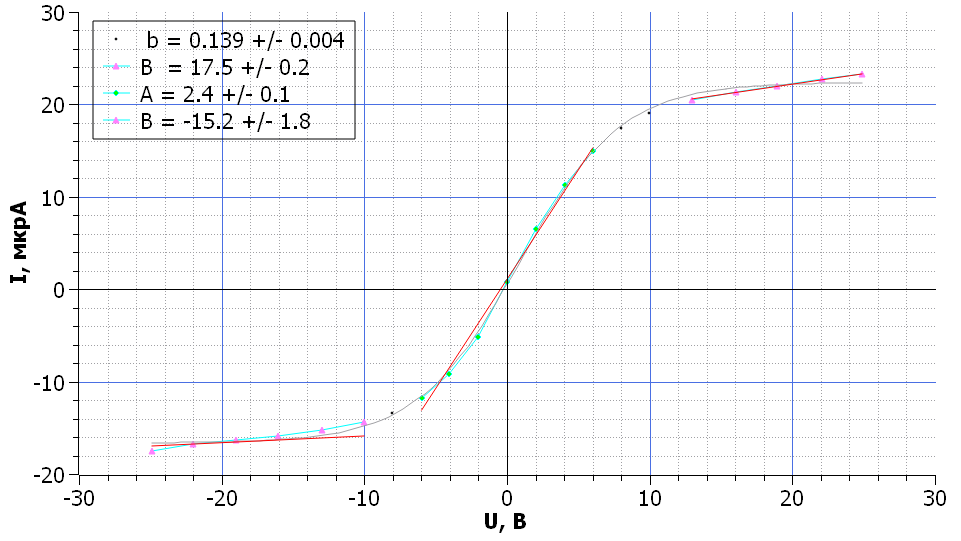
\includegraphics[scale=0.7]{ВАХ_231.png}
    \caption{ВАХ при $I_p$ = 2.31 мА}
    \label{fig:ref_to_this_foto}
\end{figure}

\par $3) \frac{dI}{dU} = (2.2 \pm 0.1) \cdot 10^6 \text{ См (Сименс)}$;
    $I_{\text{нас}} = (4.9 \pm 0.3) \cdot 10^4 \text{ СГСэ}$. \newline
Их температуры соответственно: $(3.9 \pm 0.3) \cdot 10^4 K \approx (3,4 \pm 0,3) \text{ эВ}$

\end{enumerate}
\newpage
\section{Обработка результатов}
\subsection{Обработанные данные}
\par Используя формулы (1), (2), (3), (9), (10), надём температуры электронов $T_e$ в плазме, их концентрицию $n_e$, ленгмюровсую частоту колебаний электронов $w_p$, поляризационная длина $r_{D_e}$, дебаевский радиус $r_D$, число частиц в дебаевской сфере $N_D$, и ионизацию газа $\alpha$.
\begin{table}[h!]
\centering
\begin{tabular}{|c|c|c|} \hline
$I_1$ & $\text{Величина}$   & $ \text{Погрешность, } \sigma$  \\ \hline
$T_e, 10^4 K$                          & 6,6  & 0,3                    \\ \hline
$n, 10^{10} cm^{-3}$ & 1,9  & 0,1                    \\ \hline
$w, 10^9 c^{-1}   $& 7,7  & 1,8                    \\ \hline
$r_{D_e}, 10^{-2} cm$           & 1,3  & 0,1                    \\ \hline
$r_{D}, 10^{-4} cm $             & 8,7  & 0,5                    \\ \hline
$N_D $                                                 & 52   & 9                      \\ \hline
$n, 10^{14} сm^{-3} $& 3    & 0,1                    \\ \hline
$\alpha, 10^{-3}\%  $& 6,3  & 0,4                    \\ \hline

\\ \hline

$I_2$  &    & \\ \hline
$T_e, 10^4 K      $                    & 3,7  & 0,7                    \\ \hline
$n, 10^{10} сm^{-3} $& 1,8  & 0,2                    \\ \hline
$w, 10^9 c^{-1}   $& 7,5  & 2,5                    \\ \hline
$r_{D_e}, 10^{-2} cm$           & 1    & 0,1                    \\ \hline
$r_{D}, 10^{-4} cm$              & 8,9  & 1                      \\ \hline
$N_D$ & 53   & 19             \\ \hline
$n, 10^14 сm^{-3} $& 5,3  & 1                      \\ \hline
$\alpha, 10^{-3}\%  $& 3,4  & 0,7                    \\ \hline
 \\
 \hline
$I_3$ &    & \\ \hline
$T_e, 10^4 K     $                   & 3,9  & 0,3                    \\ \hline
$n, 10^{10} сm^{-3} $& 1,4  & 0,1                    \\ \hline
$w, 10^9 c^{-1}   $& 6,6  & 1,8                    \\ \hline
$r_{D_e}, 10^{-2} cm$           & 1,2  & 0,1                    \\ \hline
$r_{D}, 10^{-4} cm $             & 10,1 & 0,7                    \\ \hline
$N_D              $                                   & 60   & 13  \\ \hline
$n, 10^{14} сm^{-3}$ & 5,1  & 0,4                    \\ \hline
$\alpha, 10^{-3} \% $  & 2,7  & 0,3                    \\ \hline
\end{tabular}
\caption{ Результаты}
\end{table}

\newpage
\subsection{Построим графики зависимости $T_e(I_p)$ и $n_e(I_p)$ по обработанным результатам}

\begin{figure}[h!]
    \centering
    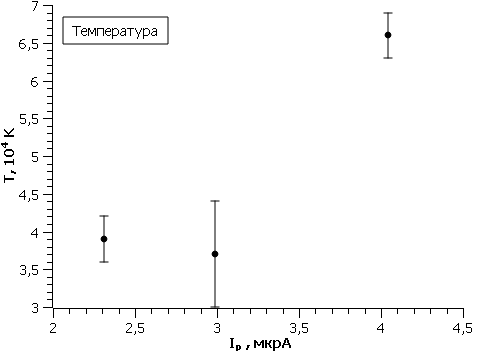
\includegraphics[scale=1.4]{T.png}
    \caption{Зависимость температуры от тока разряда}
    \label{fig:ref_to_this_foto}
\end{figure}

\begin{figure}[h!]
    \centering
    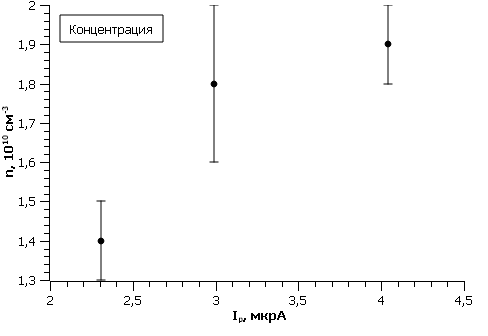
\includegraphics[scale=1.4]{n.png}
    \caption{Зависимость концентрации ионов от тока разряда}
    \label{fig:ref_to_this_foto}
\end{figure}
\newpage
\section{Выводы}
\par В данной лабораторной работе мы исследовали состояние плазмы в тлеющем газовом
разряде c помощью двойного зонда. Полученные результаты сходятся с указанными в
лабораторной работе по порядку. Плазму в тлеющем разряде можно с хорошей точностью
назвать идеальной, так как $N_D$ >> 1. Также были измерены зондовых характеристики плазмы при различных токах разряда. Полученные данные были обработаны, с их помощью было проведено исследование основных параметров плазмы –
температуры и концентрации ионов. Из того что $r_{D_e} >> r_{D_i}$ можно сделать вывод, что исследованная плазма является идеальной.


%foto
%\begin{figure}[!p]
%    \centering
%    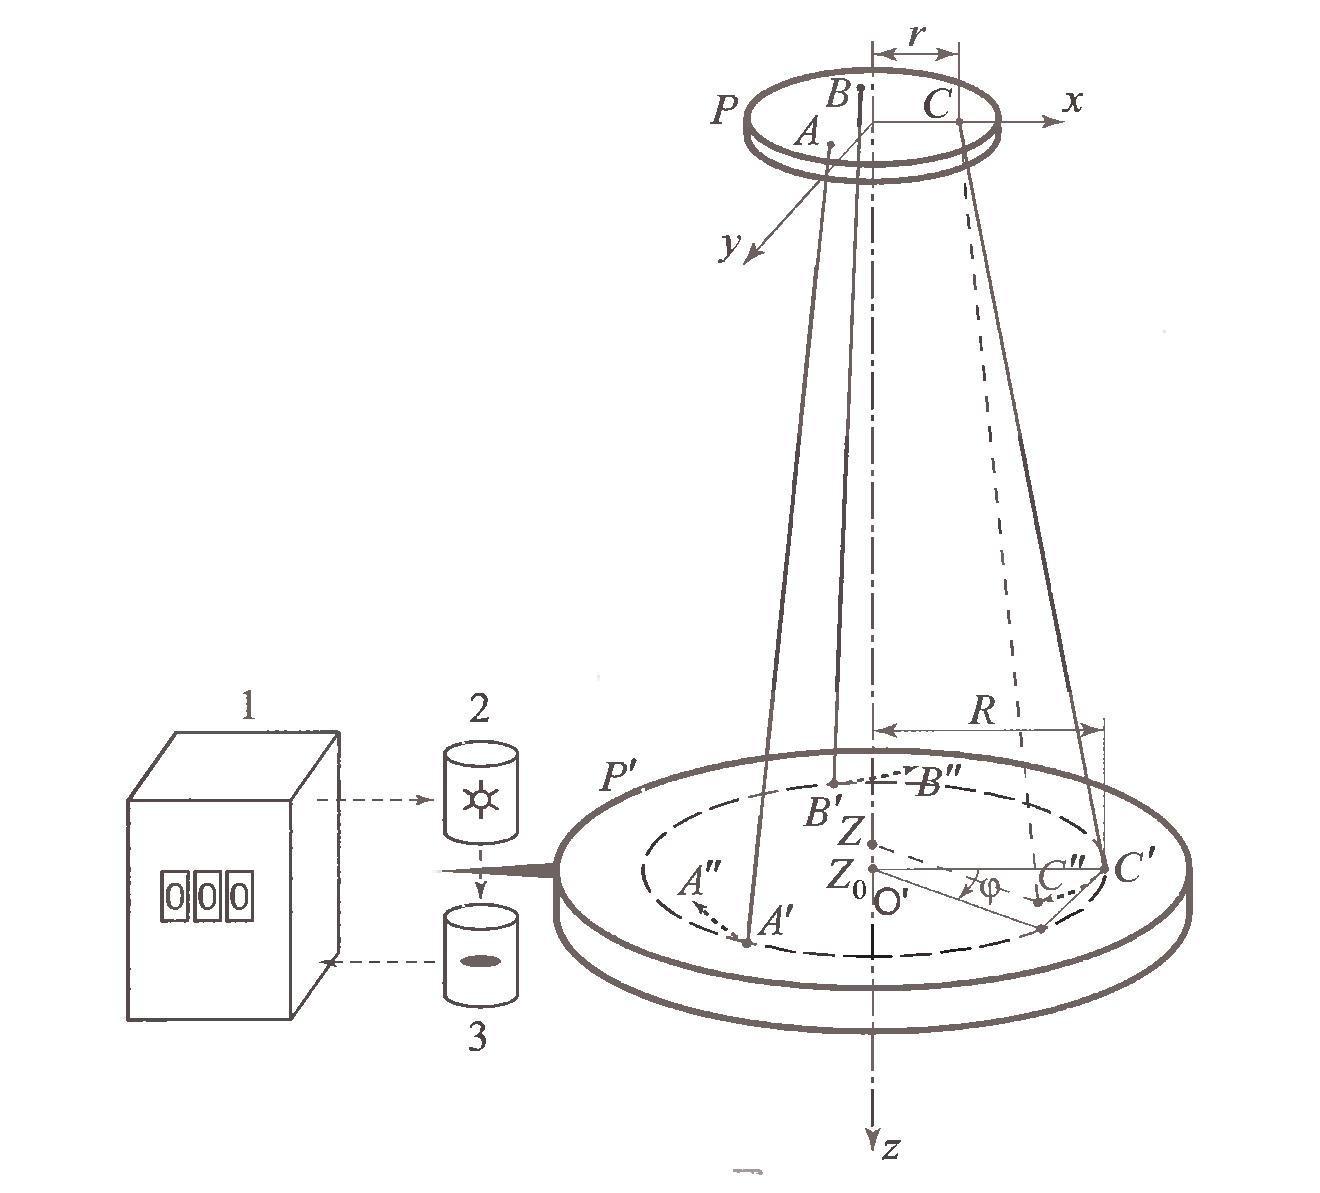
\includegraphics[scale=0.15]{foto.jpg}
%    \caption{ПНазвание}
%    \label{fig:ref_to_this_foto}
%\end{figure}

%table
%\begin{table}[!ht]
%    \centering
%    \begin{tabular}{}
%    ...
%    \end{tabular}
%    \caption{Название}
%    \label{fig:table_to_this_foto}
%\end{table}

\end{document}